\chapter{Calculation of the AC-Stark-Shift}

The calculation of the \textsc{ac}-Stark-Shift is done, using the formulas resulting from pertubation theory, as carried out in the previous sections. The first part of this chapter reviews the main results regarding the polarizabilities of the ground and first excited state. This will reveal also whether the excited state can also be trapped in the high intensity region of the lasers and how the trapping compares to that of the ground state. All calculations use the computer algebra system mathematica.\\For the meassurement, testing the theoretical foundation, that is presented in this thesis, concrete shift calculations are made regarding the big, crossed dipole trap. At the end of this section, values for the small microtrap will be presented, that will suggest, in how far the goal of imaging atoms in small traps and single sites of optical lattices can be managed. The magnetic field, and thus the quantisation axis is definde to be along the z-direction.

\section{Polarizability}
For the calculation of the polarizabilities for the respective states, the geometry and power of the used laser-beams are not important, since it only depends on the wavelength of the incoming light and on its polarization, that has a notable role for the tensor-polarizability in the vicinity of a transition resonance and renders unimportant, when using very far detuned trap-light. Before talking about concrete results, we recall the formulas given in the theory-section. 
\begin{align}
\alpha=&\left[\alpha^0_J+\frac{3m^2_J-J(J+1)}{J(2J-1)}\alpha^2_J\right]\\
\notag\\
\alpha^0_J=&\frac{2}{3(2J+1)}\sum_{K\neq J}\frac{|\braopket{J}{|r|}{K}|^2}{W_K-W_J}\notag\\
\alpha^2_J=&4C\sum_{K\neq J}(-1)^{J+K}\sixj{J}{1}{K}{1}{J}{2}\frac{|\braopket{J}{|r|}{K}|^2}{W_K-W_J}\notag
\end{align}
Following \cite{magic01}, the polarizability is calculated using atomic units (a.u.). For the calculation transitions up to $n=7$ were considered. The respective dipole-transition matrix elements are listed below, together with the energy-differences between the levels.

\begin{figure}[H]
\begin{center}
\begin{tabular}{ccc}
Transition&Matrix-element [$\unit{a.u.}$]&Resonance [$\unit{nm}$]\\\hline\hline\\
$2s_{1/2}-2p_{1/2}$&3.3169&670.791\\
$2s_{1/2}-2p_{3/2}$&4.6909&670.776\\
$2s_{1/2}-3p_{1/2}$&0.183&323.2657\\
$2s_{1/2}-3p_{3/2}$&0.259&323.2657\\
$2s_{1/2}-4p_{1/2}$&0.160&274.1203\\
$2s_{1/2}-4p_{3/2}$&0.226&274.1203\\
$2s_{1/2}-5p_{1/2}$&0.1198&256.2312\\
$2s_{1/2}-5p_{3/2}$&0.169&256.2312\\
$2s_{1/2}-6p_{1/2}$&0.0925&247.5061\\
$2s_{1/2}-6p_{3/2}$&0.131&247.5061\\
$2s_{1/2}-7p_{1/2}$&0.0737&242.5426\\
$2s_{1/2}-7p_{3/2}$&0.1042&242.5426\\
$2p_{3/2}-3s_{1/2}$&3.4403&812.645\\
$2p_{3/2}-4s_{1/2}$&0.9167&497.175\\
$2p_{3/2}-5s_{1/2}$&0.4929&427.313\\
$2p_{3/2}-6s_{1/2}$&0.3268&398.554\\
$2p_{3/2}-7s_{1/2}$&0.2397&383.564\\
$2p_{3/2}-3d_{3/2}$&2.2658&610.366\\
$2p_{3/2}-3d_{5/2}$&6.7975&670.776\\
$2p_{3/2}-4d_{3/2}$&0.8627&460.283\\
$2p_{3/2}-4d_{5/2}$&2.5882&460.289\\
$2p_{3/2}-5d_{3/2}$&0.5015&413.262\\
$2p_{3/2}-5d_{5/2}$&1.5045&413.262\\
$2p_{3/2}-6d_{3/2}$&0.3435&391.535\\
$2p_{3/2}-6d_{5/2}$&1.0306&391.535\\
$2p_{3/2}-7d_{3/2}$&0.2565&379.507\\
$2p_{3/2}-7d_{5/2}$&0.7696&379.507\\\\\hline
\end{tabular}
\end{center}
\caption{Reduced Dipole-Transition-Matrix-Elements \cite{magic01} in a.u. and the respective detuning \cite{NIST_ASD}, i.e. the resonance-energy for the relevant levels: $1s_22s_{1/2}$ and $1s_22p_{3/2}$}
\label{matrixelements}
\end{figure}
Figure \ref{alphages} shows how the polarizability behaves for different levels and different wavelength of the incoming laser-light. In this case, $\pi$-polarized light is assumed. The qualitative behaviour does not change due to different polarizations, only the magnitute of the tensor polarizability. The differences in the practical case of our experiment will be discussed later on.
\begin{figure}[H]
\centering
\begin{subfigure}[b]{0.4\textwidth}
                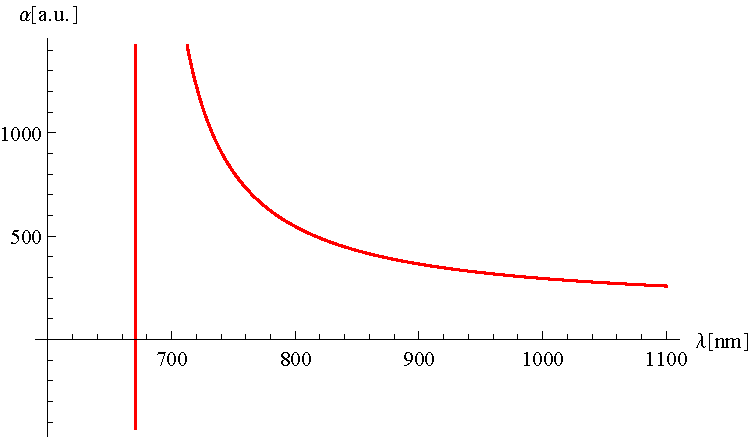
\includegraphics[width=\textwidth]{alphaground}
                \caption{$1s2s_{1/2}$}
\end{subfigure}
\begin{subfigure}[b]{0.4\textwidth}
               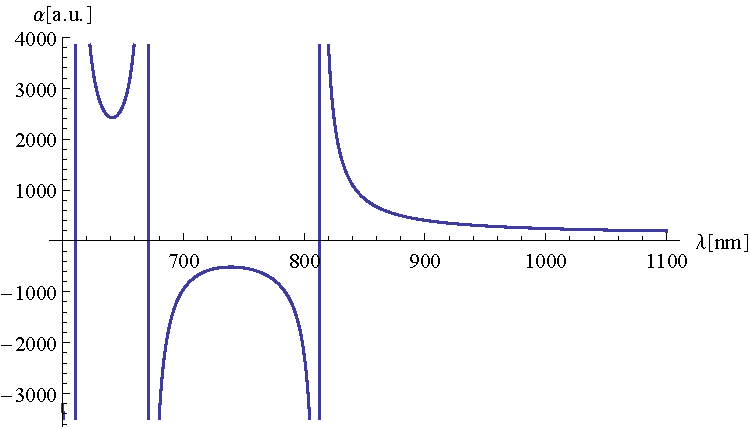
\includegraphics[width=\textwidth]{alphaexited12}
                \caption{$1s2p_{3/2}, |m_j|=1/2$}
\end{subfigure}
\begin{subfigure}[b]{0.4\textwidth}
               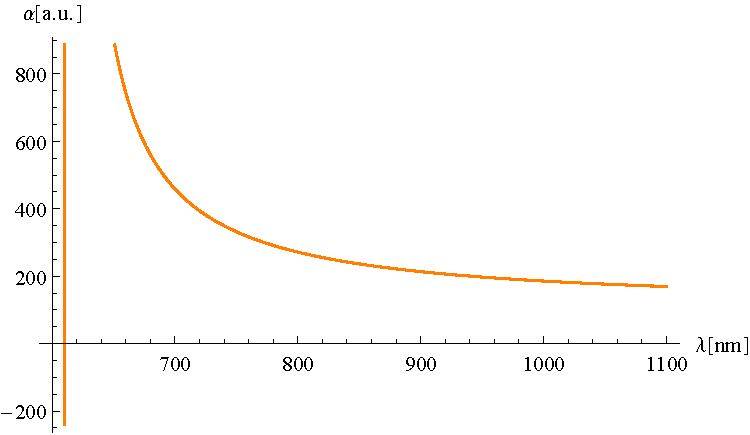
\includegraphics[width=\textwidth]{alphaexited32}
                \caption{$1s2p_{3/2}, |m_j|=3/2$}
\end{subfigure}
\begin{subfigure}[b]{0.4\textwidth}
                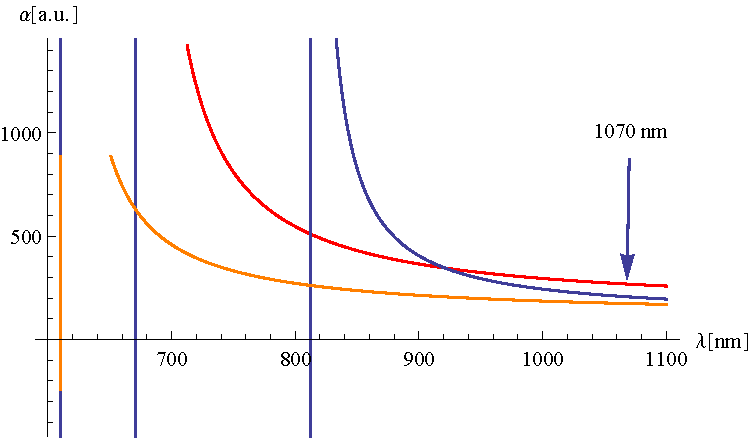
\includegraphics[width=\textwidth]{alphaalltogether}
                \caption{Comparison}
\end{subfigure}




\caption{Polarizability \alpha for the states $1s2s_{1/2}$ (red) , $1s2p_{3/2}, |m_j|=1/2$ (blue) and  $1s2p_{3/2}, |m_j|=3/2$ (orange)}
\label{alphages}
\end{figure}
What can be seen in the plots are some interesting properties. The first important result is, that, considering a far detuned light-source, the ground state, as well as the excited state show positive polarizabilities. This fundamentally contradicts the picture of a two-level system, for example described in \cite{cohen}. In this model, the excited state will be shifted in opposition to the ground state, i.e. the relative sign in the polarizability flips. This reflects the fact, that in a real atom, aspecially in the exited states of Lithium, the structure is much more complicated, than what results from the two-level approximation, because many different levels are roughly in the same energy-range and no single transtion dominates. Practically this results in the fact, that both the ground-state and the first excited states can be trapped in the same type of dipole-trap, because the positive polarizability results in a negative potential. Therefore the atoms are attracted to the highest intensity of the laser-beam. The difference lies in the exact values. For farly detuned light, i.e. above around 1000 nm of wavelength, the ground state shows a higher polarizability, than both excited states, which means, that the potential is deeper for the ground state. From figure \label{relativealpha} can be seen, how the different excited states behave relative to the ground state for the both relevant laser-wavelength for the big and the small dipole-trap in the experiment. As one could expect the difference in the regime of farly detuned light is negligible. As stated in the theory-section, the magnetic field shifts the different levels, depending on their respective angular momentum and magnetic quantum numbers. This results in different values for the detuning, that determines the polarizability. However, at 527 G, that is a high field in the framework of the experiment, the shifts due to the Zeeman-effect are very small and the overall change in the resonance is orders of magnitude below the error in predicting the differential light shift alltogether. This is an important result, thus it tells us, that in cold atom experiments, where different values of magnetic field from weak to strong are used to tune the respective interaction strength, the trapping efficiency is nearly independent from such tunings.

\begin{figure}[h]
\begin{center}
\begin{tabular}{ccc}
State&$\alpha$ at $1070\unit{nm}$ [$\unit{\alpha_{ground}}$]&$\alpha$ at $1064\unit{nm}$ [$\unit{\alpha_{ground}}$]\\\hline\hline\\
$2p_{3/2}, |m_j|=1/2$&0.7694&0.7726\\
$2p_{3/2}, |m_j|=3/2$&0.6487&0.6472\\
\\\hline
\end{tabular}
\end{center}
\caption{Polarizabilities of the excited states for the relevant laser-wavelengths, in relation to the ground state polarizability.}
\label{relativealpha}
\end{figure}

The picture looks different, when cosidering higher frequencies. There, the picture looks different, aspecially when comparing the two excited states with different magnetic quantum number. Below around 900 nm and $m_j=3/2$ the absolute value of the polarizability is much higher than for both other states. Mathematically this can easiest be seen, when looking at the formula for the total polarizability. The tensor-part of this formula is multiplied by a factor, that is -1 or +1, depending on whether $|m_j|=1/2$ or $|m_j|=3/2$. This means, that it decides whether the tensor part is added or subtracted, when calculating the total value. If it is substracted, in case of $|m_j|=3/2$, in the vicinity of many resonances, the diverging terms will cancel each other out and instead of a singularity a finite value is the result.

This does not mean, that one state can be trapped easier. When using laser-light, that is not far detuned from the respective resonances absorbtion effects cause the light to transfer momentum onto the atoms, that thus will heat up and the overall force field is no longer conervative. However using this effects in special settings can also result in effectve trapping and cooling techniques. An optical molasse for example uses a standing wave of circular polarized laser-beams, so that the electric field and thus the polarizability and the respective light-shift are spacially dependent. Using the fact, that for different $m_J$-levels the light shift is different, one can tune the different beams such that after an absorbtion cycle the atoms decay into lower $m_J$-states and thus lose energy and cool down. In an optical dipole trap however, absorbtion is an unwanted heating-effect and therefore it is most efficient, when using laser-light farly detuned from the resonances. In this regime, all magnetic sublevels strive towards the same vale of polarizability, only depending on the scalar part, that is isotropic and does not depend on the light-polarization.

\subsection{Convergence for the calculation}

\begin{figure}[H]
\centering
\begin{subfigure}[b]{0.4\textwidth}
                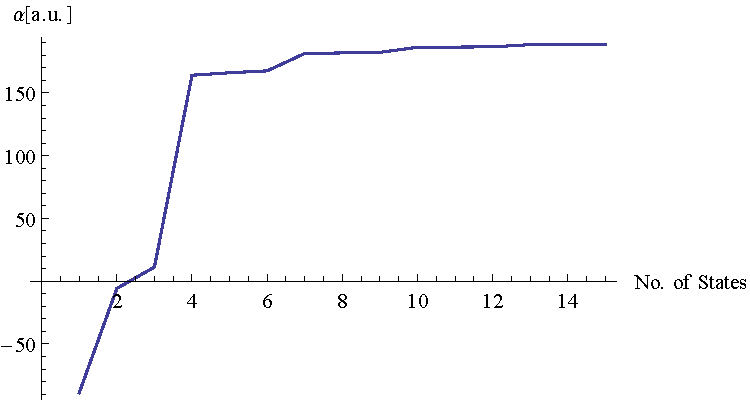
\includegraphics[width=\textwidth]{alphascalarconvexcited}
                \caption{Scalar polarizability $\alpha^0_J$}
\end{subfigure}
\begin{subfigure}[b]{0.4\textwidth}
               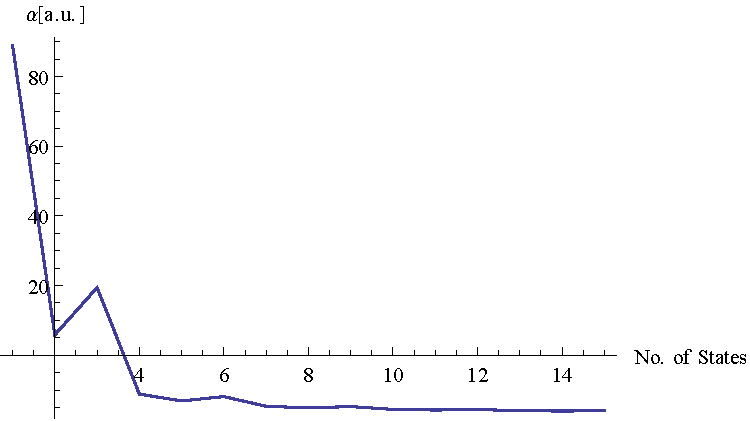
\includegraphics[width=\textwidth]{alphatensorconvexcited}
                \caption{Tensor polarizability $\alpha^2_J$}
\end{subfigure}


\caption{Convergence of the polarizability value for the excited state $1s2p_{3/2}, |m_j|=3/2$ at 1070 nm.}
\label{alphaconv}
\end{figure}

Another interesing question is, how far one has to go in calculating the energy shift in this pertubation framework to get a good approximation of the actual value. The maximum accuracy, as written above, was considering levels up to $n=7$. Figure (\ref{alphaconv}) shows how the value of $\alpha$ changes when considering higher levels. The x-coordinate is simply the index of the states, counted from low to high detuning. One can see, that for the excitet state, when going above $n=3$(Index > 4) the curve seems to converge. However for up to $n=3$, the value of $\alpha$ reaches only 85\% of its value at the full calculation. It reaches 95\% not until considering levels up to $n=5$. This is because all levels further above show little differences in detuning and also in te respective reduced matrix elements and therefore the states contribute similarily to the final result. In the case of the ground state, considering only the two lowest transitions already results in a value that has 99.8\% of the final value. Therefore the high precision calculation when taking into accound higher levels brings little benefit.

\begin{figure}[h]
\centering
\begin{subfigure}[b]{0.4\textwidth}
                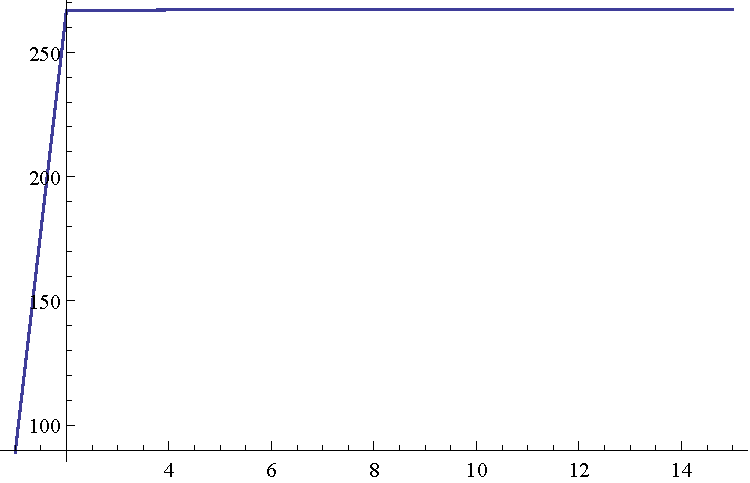
\includegraphics[width=\textwidth]{alphascalarconvground1}
                \caption{Polrizability \alpha}
\end{subfigure}
\begin{subfigure}[b]{0.4\textwidth}
               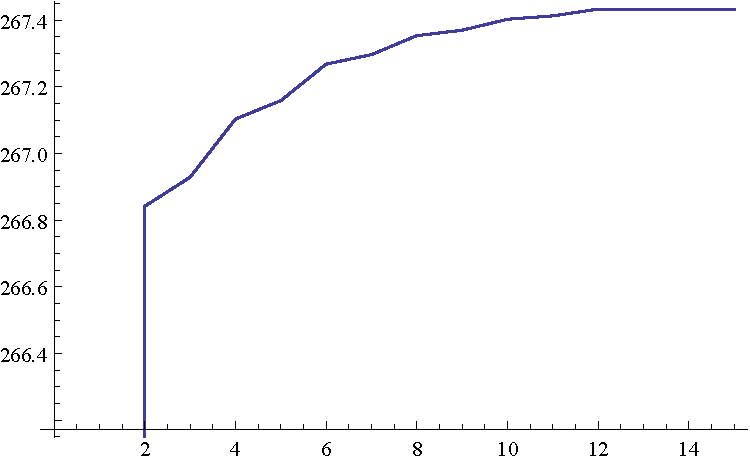
\includegraphics[width=\textwidth]{alphascalarconvground2}
                \caption{Zoom in the flat region}
\end{subfigure}


\caption{Convergence of the polarizability value for the ground state $1s2s_{1/2}$ at 1070 nm.}
\label{alphaconv2}

\end{figure}

\section{Depth of the crossed dipole trap}
\begin{figure}[H]
\centering
 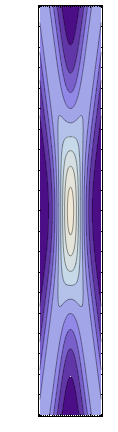
\includegraphics[width=0.3\textwidth,angle=90]{crossed_dipole_trap}

\caption{Intensity distribution for crossed dipole trap. The depth is decided by the maximum intensity in the center, that can be calculated considering a gaussian profile.}
\label{dipolegraphic}
\end{figure}

We now want to calculate the trap depth and the differential light shift, that can be meassured in the experiment. Since the ground state and the first excited states have different polarizabilities, also the light shift is varying. That means, that the energy-difference between the two states changes in case of incoming trap-light and as a result the resonance-frequency of the transition shifts, which can be much easier meassured than the actual depth of the trap. Although the crossed dipole-trap is not a single beam, the beam profile in the middle, where the intensity is at its maximum, is gaussian. That means, that like for a normal gaussian beam, the trap is characterized by its beam-power and waist. The power in this case is two times the power leaving the laser initially, since it gets reflected and forms the second beam as well. The waist in this case is 40 \mu m, with an error estimated to be around 5\%. The experiment will later be performed at multible powers, that have a much higher accuracy with an error, being roughly 0.1\%.
\begin{figure}[h]
\centering
\begin{subfigure}[b]{0.4\textwidth}
                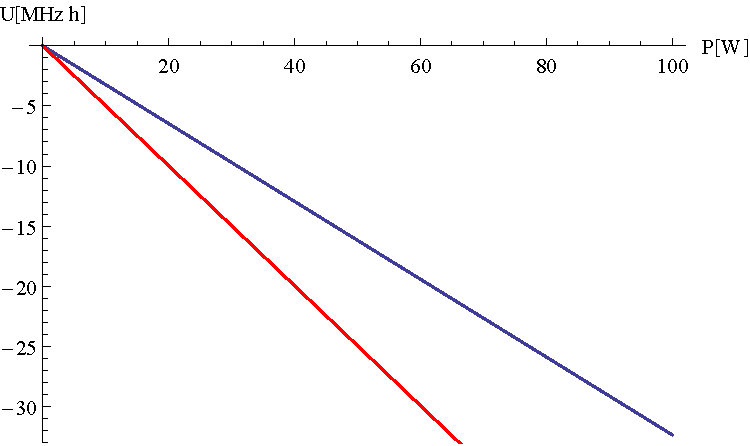
\includegraphics[width=\textwidth]{shift}
                \caption{Trap-depth for ground (red) and excited (blue) state.}
\end{subfigure}
\begin{subfigure}[b]{0.4\textwidth}
               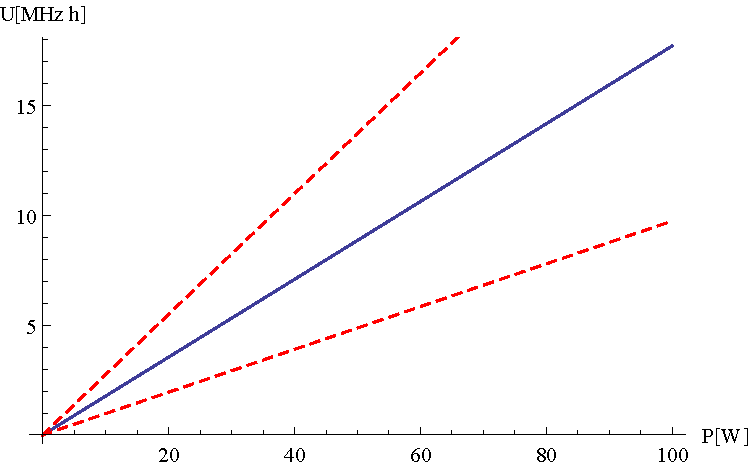
\includegraphics[width=\textwidth]{difshifterror}
                \caption{$D_2$-Resonance-Shift (blue) and the error boundary (red). Slope of $0.175\unit{MHz/W}$}
\end{subfigure}


\caption{Potential for ground ($2s$) and excited ($2p_{3/2}$$|m_J|=3/2$) state and the difference of both, i.e. the shift of the D2-resonance, for different total powers of the trap-beam.}
\label{potential}
\end{figure}


\subsection{Magnetic Field}



%\begin{figure}[h]
%\begin{center}
%\begin{tabular}{cccc}
%Transition&$\Delta E_\delta [\unit{MHz}\ h]$&$\Delta E_\delta$ at $572\unit{G}  [\unit{MHz }\ h]$&$\Delta\Delta E_\delta [\unit{MHz }\ h]$\\\hline\hline\\
%$2s\rightarrow 2p_{3/2}, |m_j|=1/2$&2.87545&2.87538&1.58106\\
%$2s\rightarrow 2p_{3/2}, |m_j|=3/2$&4.38047&4.38050&1.29365\\
%\\\hline
%\end{tabular}
%\end{center}
%\caption{Differential \textsc{ac}-Stark shift at 50 W of total beam power with and without magnetic field. The sensitivity to the waist-uncertainty leads to a large error and to irrelevance of the magnetic field.}
%\label{relativealpha}
%\end{figure}


\section{Comparison to the classical formula}

Since the classical formula in (\ref{classic}) is widely used to calculate depths for optical dipole traps it is interesting to see, in how far it differs from the quantum-mechanical approach. For the excited state, for allready stated reasons, it is not possible to calculate a good value using this approach, but the ground state, for that the coupling to other states is dominated by the transition to the first excited state, the formula gives values, that differ only 0.3\% when calculating the shift considering transitions up to $n=7$ and using 1070 nm light. When only considering the D-Line transition, both values are the same in range and differ about 0.01 \%. That shows, that using the approach of a harmonic oscillator to model the dipole-trap potential gives good results, when dealing with a system that can be approximated to only consist of two states. In the case of the Lithium-6 ground state, where for infrared light and higher excited states the transitions are very farly detuned, the model gives a good estimate, that is less complicated to calculate than the approach of pertubation theory.